\begin{CJK}{Bg5}{bsmi}

%---------------------------------------------
%	Chapter Discussion
%---------------------------------------------

\chapter{Discussion}

\section{Security Analysis}

\begin{comment}
This is the most important part of an authentication system.
We have to define our threat model before we start to analyze.
There are 4 components in the scheme I proposed.
\end{comment}

\subsection{Threat Model}

\subsubsection{Secure Object}

In my system, the most important goal is to protect user's privacy, that is, attackers cannot pretend to be the real user. To achieve the goal, we cannot leak any information about users' private key. Futhermore, attackers shouldn't get nonce and signed-nonce at same time.

\subsubsection{Trust Boundary}

There are 5 components in this scheme, and 4 possible channels for data transfer, as the fig~\ref{fig:compose-element} shows. Because the mobile device is a private accessories, I assumed that the mobile device is trusted, that is, it is a unrooted Android phone with a secure data storage. No one can dump the memory out or cahnged any value saved in storage. 

\begin{figure}
\centering
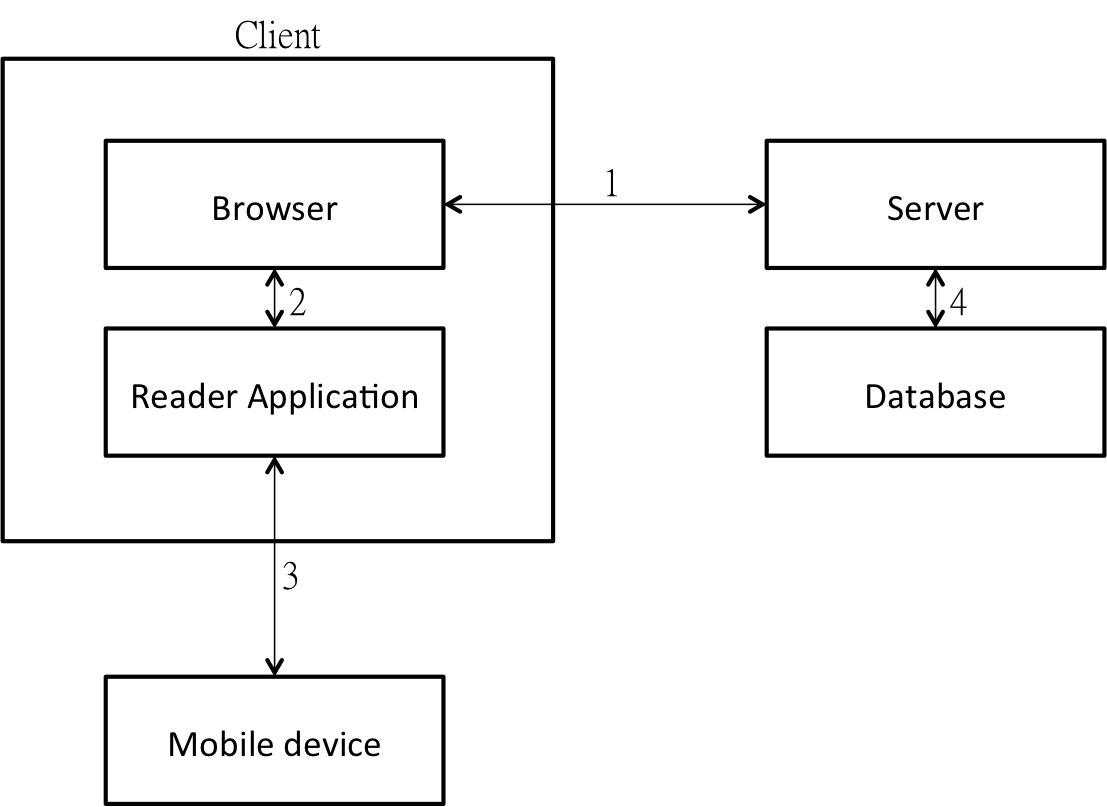
\includegraphics[scale=0.6]{picture/compose-element.png}
\caption{Components}
\label{fig:compose-element}
\end{figure}

The browser and the reader applicaiton are usually on the same PC, so we can view these two parts as a same component. However, our PC is vulnerable due to spreading virus and malicious program. Our keyboard may be logger, nevertheless, the communication channels between client and either mobile device or server is not secure. To be clearer, even though I adopt HTTPS for the network channel, the data which transfered on these channel may be sniffed or even modified. The last component is the server side. In my assumption, the server is secure enough, attackers can only read the data saved in the databased but cannot modified.

\subsubsection{Threats}

In this paragraph, I'll discuss the possible threats and weaknesses that could affect my system under this assumption. Futhermore, I'll compare my scehem to the original password-based scheme, to see the improvement of my new design.

First, due to the mobile device is secure, so it is impossible of any attacks on mobile device. Then we discuss the attack on client side (browser and reader applicaiton). For password-based scheme, malicious people can easily get password by any physical attack such as key-logged attack. The network communication is insecure, and we can not trust the server's certificate, so this authentication system will under phishing attack and the Man-In-The-Middle attack with password-based scheme. Next, consider an authetication system with my scheme, all attacks to client side is useless, its because these attack can only get signed-nonce or public key, which do not leak any information about the private key. Unfortunately, my scheme has no resistance to phishing attack and MITM attack, because of the insecure network channel. However, there is another advantage of my scheme. Even though there is an attacker get the authority in one authentication process, the attacker will not be able to use this information on another authentication process. Unlike password-based scheme, if a attacker get your password, then he can pretend to be the real user any time.

Last, for the attacks on the server side. Under my assumption, attackers can only read the data saved in database. For password-based scheme, it is a little dangerous for users. If the users' credentials are saved in plaintext, then the attackers will know everythings he wants. Even though it saved after encrypt, there still is in the risk that the key is found by attackers. To sum up, password-based scheme is still not secure enough under this assumption. Comparatively, for my scheme, the data saved in server are the UUID and the public key, which cause no any effect to users' privacy.

\section{Usability Analysis}

\subsection{Criterias}

\subsubsection{Memorywise-effort}

This criteria means that how many things a user has to remember when he adopt this scheme. Take password-based scheme as an example, the memorywise-effort is username and password. A scheme with less memorywise effort can get higher score in this criteria.

\subsubsection{Scalable-for-user}

Will this scheme create burden for users? The \emph{scalable} is from the viewpoint of users.

\subsubsection{Nothing-to-carry}

Users do not need to bring anything if they adopt this scheme.

\subsubsection{Physical-effortless}

This criteria means that how many effort should a user do in an authentication process.

\subsubsection{Efficiency}

Efficiency means the during time of an authenticaiton process. Not only the calculating time, it should also include the operating time. For example, if a user need to enter an OTP himself, then this scheme is not efficiency.

\subsubsection{Infrequent-error}

Infrequent-error means this scheme or system must be reliable. It cannot reject an authentication request to a honest user.

\subsubsection{Easy-recovery-from-loss}

Users can regain the authentication ability if they lost their devices or if they forgot the needed credentials.

\subsection{Analysis}

\begin{comment}
The usability can not be neglected when researchers trying to design a system.
Usability is a subjective perception, it may be different from person to person.
The following paragragh states the criterias I used to estimate the usability of a system.
\end{comment}

\section{Deployment Ability Analysis}

\subsection{Criterias}

\subsubsection{Accessible}

User who adopt this scheme will not be constrained by disabilities or any other physical conditions.

\subsubsection{User-cost}

The total cost per user of the scheme. It should including both required devices of client-side and required equipment of the verification server.

\subsubsection{Server-compatable}

From the viewpoint of verification server, the scheme is compatable with the text-based passwords. The server will not need change their setup to support this scheme. 

\subsubsection{Browser-compatable}

Users don't have to change anything to support this scheme. 

\subsection{Analysis}

\begin{comment}
The deployment ability is also an important thing which is need to be considered, especially in designing an authentication system.
A system with high usability means it is friendly to users; a system with high deployment ability means it is friendly to the system provider or, more precise, the developers.
The following paragraph states the criterias I used to estimate a system's deployment ability. 
\end{comment}


\end{CJK}